% TODO translate
\subsection{Simple encryption using XOR mask}
\label{XOR_mask_1}

I've found an old interactive fiction game while diving deep into \IT{if-archive}\footnote{\url{http://www.ifarchive.org/}}:

\begin{lstlisting}
The New Castle v3.5 - Text/Adventure Game
in the style of the original Infocom (tm)
type games, Zork, Collosal Cave (Adventure),
etc.  Can you solve the mystery of the
abandoned castle?
Shareware from Software Customization.
Software Customization [ASP] Version 3.5 Feb. 2000
\end{lstlisting}

It's downloadable here: \url{https://github.com/DennisYurichev/RE-for-beginners/blob/master/ff/XOR/mask_1/files/newcastle.tgz}.

There is a file inside (named \IT{castle.dbf}) which is clearly encrypted, but not by a real crypto algorithm, nor it's compressed, this is something rather simpler.
I wouldn't even measure entropy level (\myref{entropy}) of the file, because I'm sure it's low.
Here is how it looks like in Midnight Commander:

\begin{figure}[H]
\centering
\myincludegraphics{ff/XOR/mask_1/mc_encrypted.png}
\caption{Encrypted file in Midnight Commander}
\end{figure}

The encrypted file can be downloaded here:
\url{https://github.com/DennisYurichev/RE-for-beginners/blob/master/ff/XOR/mask_1/files/castle.dbf.bz2}.

Will it be possible to decrypt it without accessing to the program, using just this file?

There is a clearly visible pattern of repeating string.
If a simple encryption by XOR mask was applied, such repeating strings is a prominent signature,
because, probably, there were a long lacunas of zero bytes,
which, in turn, are present in many executable files as well as in binary data files.

\myindex{UNIX!xxd}
Here I'll dump the file's beginning using \IT{xxd} UNIX utility:

\lstinputlisting{ff/XOR/mask_1/xxd_result.txt}

Let's stick at visible repeating \TT{iubgv} string.
By looking at this dump, we can clearly see that the period of the string occurrence is 0x51 or 81.
Probably, 81 is size of block?
The size of the file is 1658961, and it can be divided evenly by 81 (and there are 20481 blocks then).

Now I'll use Mathematica to analyze, are there repeating 81-byte blocks in the file?
I'll split input file by 81-byte blocks and then I'll use 
\IT{Tally[]}\footnote{\url{https://reference.wolfram.com/language/ref/Tally.html}}
function which just counts, how many times some item has been occurred in the input list.
Tally's output is not sorted, so I also add \IT{Sort[]} function to sort it by number of occurrences in descending order.

\begin{lstlisting}[style=custommath]
input = BinaryReadList["/home/dennis/.../castle.dbf"];

blocks = Partition[input, 81];

stat = Sort[Tally[blocks], #1[[2]] > #2[[2]] &]
\end{lstlisting}

And here is output:

\begin{lstlisting}[style=custommath]
{{{80, 103, 2, 116, 113, 102, 118, 25, 99, 8, 19, 23, 116, 125, 107, 
   25, 99, 109, 114, 102, 14, 121, 115, 31, 9, 117, 113, 111, 5, 4, 
   127, 28, 122, 101, 8, 110, 14, 18, 124, 106, 16, 20, 104, 119, 8, 
   109, 26, 106, 9, 97, 13, 99, 15, 119, 20, 105, 117, 98, 103, 118, 
   1, 126, 29, 97, 122, 17, 15, 114, 110, 3, 5, 125, 125, 99, 126, 
   119, 102, 30, 122, 2, 117}, 1739}, 
{{80, 100, 2, 116, 113, 102, 118, 25, 99, 8, 19, 23, 116, 
   125, 107, 25, 99, 109, 114, 102, 14, 121, 115, 31, 9, 117, 113, 
   111, 5, 4, 127, 28, 122, 101, 8, 110, 14, 18, 124, 106, 16, 20, 
   104, 119, 8, 109, 26, 106, 9, 97, 13, 99, 15, 119, 20, 105, 117, 
   98, 103, 118, 1, 126, 29, 97, 122, 17, 15, 114, 110, 3, 5, 125, 
   125, 99, 126, 119, 102, 30, 122, 2, 117}, 1422}, 
{{80, 101, 2, 116, 113, 102, 118, 25, 99, 8, 19, 23, 116, 
   125, 107, 25, 99, 109, 114, 102, 14, 121, 115, 31, 9, 117, 113, 
   111, 5, 4, 127, 28, 122, 101, 8, 110, 14, 18, 124, 106, 16, 20, 
   104, 119, 8, 109, 26, 106, 9, 97, 13, 99, 15, 119, 20, 105, 117, 
   98, 103, 118, 1, 126, 29, 97, 122, 17, 15, 114, 110, 3, 5, 125, 
   125, 99, 126, 119, 102, 30, 122, 2, 117}, 1012},
{{80, 120, 2, 116, 113, 102, 118, 25, 99, 8, 19, 23, 116, 
   125, 107, 25, 99, 109, 114, 102, 14, 121, 115, 31, 9, 117, 113, 
   111, 5, 4, 127, 28, 122, 101, 8, 110, 14, 18, 124, 106, 16, 20, 
   104, 119, 8, 109, 26, 106, 9, 97, 13, 99, 15, 119, 20, 105, 117, 
   98, 103, 118, 1, 126, 29, 97, 122, 17, 15, 114, 110, 3, 5, 125, 
   125, 99, 126, 119, 102, 30, 122, 2, 117}, 377},

...

{{80, 2, 74, 49, 113, 21, 62, 88, 39, 71, 68, 23, 63, 51, 36, 78, 48, 
   108, 114, 102, 14, 121, 115, 31, 9, 117, 113, 111, 5, 4, 127, 28, 
   122, 101, 8, 110, 14, 18, 124, 106, 16, 20, 104, 119, 8, 109, 26, 
   106, 9, 97, 13, 99, 15, 119, 20, 105, 117, 98, 103, 118, 1, 126, 
   29, 97, 122, 17, 15, 114, 110, 3, 5, 125, 125, 99, 126, 119, 102, 
   30, 122, 2, 117}, 1},
{{80, 1, 74, 59, 113, 45, 56, 86, 52, 91, 19, 64, 60, 60, 63, 
   25, 38, 59, 59, 42, 14, 53, 38, 77, 66, 38, 113, 38, 75, 4, 43, 84,
    63, 101, 64, 43, 79, 64, 40, 57, 16, 91, 46, 119, 69, 40, 84, 117,
    9, 97, 13, 99, 15, 119, 20, 105, 117, 98, 103, 118, 1, 126, 29, 
   97, 122, 17, 15, 114, 110, 3, 5, 125, 125, 99, 126, 119, 102, 30, 
   122, 2, 117}, 1},
{{80, 2, 74, 49, 113, 49, 51, 92, 39, 8, 92, 81, 116, 62, 57, 
   80, 46, 40, 114, 36, 75, 56, 33, 76, 9, 55, 56, 59, 81, 65, 45, 28,
    60, 55, 93, 39, 90, 28, 124, 106, 16, 20, 104, 119, 8, 109, 26, 
   106, 9, 97, 13, 99, 15, 119, 20, 105, 117, 98, 103, 118, 1, 126, 
   29, 97, 122, 17, 15, 114, 110, 3, 5, 125, 125, 99, 126, 119, 102, 
   30, 122, 2, 117}, 1}}
\end{lstlisting}

Tally's output is a list of pairs, each pair has 81-byte block and number of times it has been occurred in the file.
We see that the most frequent block is the first, it has been occurred 1739 times.
The second one has been occurred 1422 times. There are others: 1012 times, 377 times, etc.
81-byte blocks which has been occurred just once are at the end of output.

Let's try to compare these blocks. The first and the second.
Is there a function in Mathematica which compares lists/arrays?
Certainly is, but for educational purposes, I'll use XOR operation for comparison.
Indeed: if bytes in two input arrays are identical, XOR result is 0. If they are non-equal, result will be non-zero.

Let's compare first block (occurred 1739 times) and the second (occurred 1422 times):

\begin{lstlisting}[style=custommath]
In[]:= BitXor[stat[[1]][[1]], stat[[2]][[1]]]
Out[]= {0, 3, 0, 0, 0, 0, 0, 0, 0, 0, 0, 0, 0, 0, 0, 0, 0, 0, 0, \
0, 0, 0, 0, 0, 0, 0, 0, 0, 0, 0, 0, 0, 0, 0, 0, 0, 0, 0, 0, 0, 0, 0, \
0, 0, 0, 0, 0, 0, 0, 0, 0, 0, 0, 0, 0, 0, 0, 0, 0, 0, 0, 0, 0, 0, 0, \
0, 0, 0, 0, 0, 0, 0, 0, 0, 0, 0, 0, 0, 0, 0, 0}
\end{lstlisting}

They are differ only in the second byte.

Let's compare the second block (occurred 1422 times) and the third (occurred 1012 times):

\begin{lstlisting}[style=custommath]
In[]:= BitXor[stat[[2]][[1]], stat[[3]][[1]]]
Out[]= {0, 1, 0, 0, 0, 0, 0, 0, 0, 0, 0, 0, 0, 0, 0, 0, 0, 0, 0, \
0, 0, 0, 0, 0, 0, 0, 0, 0, 0, 0, 0, 0, 0, 0, 0, 0, 0, 0, 0, 0, 0, 0, \
0, 0, 0, 0, 0, 0, 0, 0, 0, 0, 0, 0, 0, 0, 0, 0, 0, 0, 0, 0, 0, 0, 0, \
0, 0, 0, 0, 0, 0, 0, 0, 0, 0, 0, 0, 0, 0, 0, 0}
\end{lstlisting}

They are also differ only in the second byte.

Anyway, let's try to use the most occurred block as a XOR key and try to decrypt four first 81-byte blocks in the file:

\begin{lstlisting}[style=custommath]
In[]:= key = stat[[1]][[1]]
Out[]= {80, 103, 2, 116, 113, 102, 118, 25, 99, 8, 19, 23, 116, \
125, 107, 25, 99, 109, 114, 102, 14, 121, 115, 31, 9, 117, 113, 111, \
5, 4, 127, 28, 122, 101, 8, 110, 14, 18, 124, 106, 16, 20, 104, 119, \
8, 109, 26, 106, 9, 97, 13, 99, 15, 119, 20, 105, 117, 98, 103, 118, \
1, 126, 29, 97, 122, 17, 15, 114, 110, 3, 5, 125, 125, 99, 126, 119, \
102, 30, 122, 2, 117}

In[]:= ToASCII[val_] := If[val == 0, " ", FromCharacterCode[val, "PrintableASCII"]]

In[]:= DecryptBlockASCII[blk_] := Map[ToASCII[#] &, BitXor[key, blk]]

In[]:= DecryptBlockASCII[blocks[[1]]]
Out[]= {" ", " ", " ", " ", " ", " ", " ", " ", " ", " ", " ", " \
", " ", " ", " ", " ", " ", " ", " ", " ", " ", " ", " ", " ", " ", " \
", " ", " ", " ", " ", " ", " ", " ", " ", " ", " ", " ", " ", " ", " \
", " ", " ", " ", " ", " ", " ", " ", " ", " ", " ", " ", " ", " ", " \
", " ", " ", " ", " ", " ", " ", " ", " ", " ", " ", " ", " ", " ", " \
", " ", " ", " ", " ", " ", " ", " ", " ", " ", " ", " ", " ", " "}

In[]:= DecryptBlockASCII[blocks[[2]]]
Out[]= {" ", "e", "H", "E", " ", "W", "E", "E", "D", " ", "O", \
"F", " ", "C", "R", "I", "M", "E", " ", "B", "E", "A", "R", "S", " ", \
"B", "I", "T", "T", "E", "R", " ", "F", "R", "U", "I", "T", "?", \
" ", " ", " ", " ", " ", " ", " ", " ", " ", " ", " ", " ", " ", " ", \
" ", " ", " ", " ", " ", " ", " ", " ", " ", " ", " ", " ", " ", " ", \
" ", " ", " ", " ", " ", " ", " ", " ", " ", " ", " ", " ", " ", " ", \
" "}

In[]:= DecryptBlockASCII[blocks[[3]]]
Out[]= {" ", "?", " ", " ", " ", " ", " ", " ", " ", " ", " \
", " ", " ", " ", " ", " ", " ", " ", " ", " ", " ", " ", " ", " ", " \
", " ", " ", " ", " ", " ", " ", " ", " ", " ", " ", " ", " ", " ", " \
", " ", " ", " ", " ", " ", " ", " ", " ", " ", " ", " ", " ", " ", " \
", " ", " ", " ", " ", " ", " ", " ", " ", " ", " ", " ", " ", " ", " \
", " ", " ", " ", " ", " ", " ", " ", " ", " ", " ", " ", " ", " ", " \
"}

In[]:= DecryptBlockASCII[blocks[[4]]]
Out[]= {" ", "f", "H", "O", " ", "K", "N", "O", "W", "S", " ", \
"W", "H", "A", "T", " ", "E", "V", "I", "L", " ", "L", "U", "R", "K", \
"S", " ", "I", "N", " ", "T", "H", "E", " ", "H", "E", "A", "R", "T", \
"S", " ", "O", "F", " ", "M", "E", "N", "?", " ", " ", " ", " ", \
" ", " ", " ", " ", " ", " ", " ", " ", " ", " ", " ", " ", " ", " ", \
" ", " ", " ", " ", " ", " ", " ", " ", " ", " ", " ", " ", " ", " ", \
" "}
\end{lstlisting}

(I've replaced unprintable characters by \q{?}.)

So we see that the first and the third blocks are empty (or almost empty),
but the second and the fourth has clearly visible English language words/phrases.
It seems that our assumption about key is correct (at least partially).
This means that the most occurred 81-byte block in the file can be found at places of lacunas
of zero bytes or something like that.

Let's try to decrypt the whole file:

\begin{lstlisting}[style=custommath]
DecryptBlock[blk_] := BitXor[key, blk]

decrypted = Map[DecryptBlock[#] &, blocks];

BinaryWrite["/home/dennis/.../tmp", Flatten[decrypted]]

Close["/home/dennis/.../tmp"]
\end{lstlisting}

\begin{figure}[H]
\centering
\myincludegraphics{ff/XOR/mask_1/mc_decrypted1.png}
\caption{Decrypted file in Midnight Commander, 1st attempt}
\end{figure}

Looks like some kind of English phrases from some game, but something wrong.
First of all, cases are inverted: phrases and some words are started with lowercase characters,
while other characters are in upper case.
Also, some phrases started with wrong letters.
Take a look at the very first phrase: \q{eHE WEED OF CRIME BEARS BITTER FRUIT}.
What is \q{eHE}? Isn't \q{tHE} have to be here?
Is it possible that our decryption key has wrong byte at this place?

Let's look again at the second block in the file, at key and at decryption result:

\begin{lstlisting}[style=custommath]
In[]:= blocks[[2]]
Out[]= {80, 2, 74, 49, 113, 49, 51, 92, 39, 8, 92, 81, 116, 62, \
57, 80, 46, 40, 114, 36, 75, 56, 33, 76, 9, 55, 56, 59, 81, 65, 45, \
28, 60, 55, 93, 39, 90, 28, 124, 106, 16, 20, 104, 119, 8, 109, 26, \
106, 9, 97, 13, 99, 15, 119, 20, 105, 117, 98, 103, 118, 1, 126, 29, \
97, 122, 17, 15, 114, 110, 3, 5, 125, 125, 99, 126, 119, 102, 30, \
122, 2, 117}

In[]:= key
Out[]= {80, 103, 2, 116, 113, 102, 118, 25, 99, 8, 19, 23, 116, \
125, 107, 25, 99, 109, 114, 102, 14, 121, 115, 31, 9, 117, 113, 111, \
5, 4, 127, 28, 122, 101, 8, 110, 14, 18, 124, 106, 16, 20, 104, 119, \
8, 109, 26, 106, 9, 97, 13, 99, 15, 119, 20, 105, 117, 98, 103, 118, \
1, 126, 29, 97, 122, 17, 15, 114, 110, 3, 5, 125, 125, 99, 126, 119, \
102, 30, 122, 2, 117}

In[]:= BitXor[key, blocks[[2]]]
Out[]= {0, 101, 72, 69, 0, 87, 69, 69, 68, 0, 79, 70, 0, 67, 82, \
73, 77, 69, 0, 66, 69, 65, 82, 83, 0, 66, 73, 84, 84, 69, 82, 0, 70, \
82, 85, 73, 84, 14, 0, 0, 0, 0, 0, 0, 0, 0, 0, 0, 0, 0, 0, 0, 0, 0, \
0, 0, 0, 0, 0, 0, 0, 0, 0, 0, 0, 0, 0, 0, 0, 0, 0, 0, 0, 0, 0, 0, 0, \
0, 0, 0, 0}
\end{lstlisting}

Encrypted byte is 2, the byte from the key is 103, $2 \oplus 103=101$ and 101 is ASCII code for \q{e} character.
What byte of a key must be equal to, so the resulting ASCII code will be 116 (for \q{t} character)?
$2 \oplus 116=118$, let's put 118 in key at the second byte \dots

\begin{lstlisting}[style=custommath]
key = {80, 118, 2, 116, 113, 102, 118, 25, 99, 8, 19, 23, 116, 125, 
  107, 25, 99, 109, 114, 102, 14, 121, 115, 31, 9, 117, 113, 111, 5, 
  4, 127, 28, 122, 101, 8, 110, 14, 18, 124, 106, 16, 20, 104, 119, 8,
   109, 26, 106, 9, 97, 13, 99, 15, 119, 20, 105, 117, 98, 103, 118, 
  1, 126, 29, 97, 122, 17, 15, 114, 110, 3, 5, 125, 125, 99, 126, 119,
   102, 30, 122, 2, 117}
\end{lstlisting}

\dots and decrypt the whole file again.

\begin{figure}[H]
\centering
\myincludegraphics{ff/XOR/mask_1/mc_decrypted2.png}
\caption{Decrypted file in Midnight Commander, 2nd attempt}
\end{figure}

Wow, now the grammar is correct, all phrases started with correct letters.
But still, case inversion is suspicious.
Why would game's developer write them in such a manner?
Maybe our key is still incorrect?

While observing ASCII table we can notice that uppercase and lowercase letter's ASCII codes are differ in just one bit
(6th bit starting at 1st, 0b100000):

\begin{figure}[H]
\centering
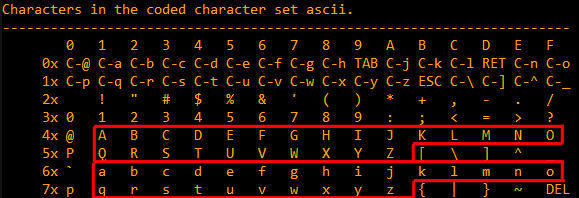
\includegraphics[width=0.7\textwidth]{ascii.png}
\caption{7-bit \ac{ASCII} table in Emacs}
\end{figure}

This bit in decimal form is 32 \dots 32?
But 32 is ASCII code for space!

Indeed, one can switch case just by XOR-ing ASCII character code with 32 (more about it: \myref{toupper_bit}).

It is possible that the empty lacunas in the file are not zero bytes, but rather spaces?
Let's modify XOR key one more time (I'll XOR each byte of key by 32):

\begin{lstlisting}[style=custommath]
(* "32" is scalar and "key" is vector, but that's OK *)

In[]:= key3 = BitXor[32, key]
Out[]= {112, 86, 34, 84, 81, 70, 86, 57, 67, 40, 51, 55, 84, 93, 75, \
57, 67, 77, 82, 70, 46, 89, 83, 63, 41, 85, 81, 79, 37, 36, 95, 60, \
90, 69, 40, 78, 46, 50, 92, 74, 48, 52, 72, 87, 40, 77, 58, 74, 41, \
65, 45, 67, 47, 87, 52, 73, 85, 66, 71, 86, 33, 94, 61, 65, 90, 49, \
47, 82, 78, 35, 37, 93, 93, 67, 94, 87, 70, 62, 90, 34, 85}

In[]:= DecryptBlock[blk_] := BitXor[key3, blk]
\end{lstlisting}

Let's decrypt the input file again:

\begin{figure}[H]
\centering
\myincludegraphics{ff/XOR/mask_1/mc_decrypted.png}
\caption{Decrypted file in Midnight Commander, final attempt}
\end{figure}

(Decrypted file is available here:
\url{https://github.com/DennisYurichev/RE-for-beginners/blob/master/ff/XOR/mask_1/files/decrypted.dat.bz2}.)

This is undoubtedly a correct source file.
Oh, and we see numbers at the start of each block. It has to be a source of our erroneous XOR key.
As it seems, the most occurred 81-byte block in the file is a block filled with spaces and containing \q{1} character at the place of second byte.
Indeed, somehow, many blocks here are interleaved with this one.
Maybe it's some kind of padding for short phrases/messages?
Other frequently occurred 81-byte blocks are also space-filled blocks, but with different digit,
hence, they are differ only at the second byte.

That's all! Now we can write an utility to encrypt the file back, and maybe modify it before.

Mathematica notebook file is downloadable here:
\url{https://github.com/DennisYurichev/RE-for-beginners/blob/master/ff/XOR/mask_1/files/XOR_mask_1.nb}.

Summary: XOR encryption like that is not robust at all. It has been intended by game's developer(s), probably, just to prevent gamer(s) to peek into internals of game, nothing else more serious.
Still, encryption like that is extremely popular due to its simplicity and many reverse engineers are usually familiar with it.

